\chapter{Diskussion}\label{chap:diskussion}

Ziel dieser Arbeit war die Entwicklung eines Modells zur \gls{VHF}-Detektion im \gls{EKG}, das robust gegen veränderte Signalmorphologie ist. Dazu wurden 3 Modelle (\gls{DANN}, DANNdirect und InceptionTime) trainiert und auf Daten der Quell- und der Zieldomäne getestet. Die entsprechenden Ergebnisse werden in diesem Kapitel eingeordnet und diskutiert. In \hyperref[sec:einordnung]{Abschnitt 7.1} wird zunächst die Klassifikationsgüte der Modelle auf der Quelldomäne eingeordnet. In \hyperref[sec:diskhyper]{Abschnitt 7.2} werden die Ergebnisse der Hyperparameteroptimierung und in \hyperref[sec:disktest]{Abschnitt 7.3} die Ergebnisse auf den Testdatensätzen diskutiert. Zuletzt wird in \hyperref[sec:disknorm]{Abschnitt 7.4} der Einfluss von Normalisierung diskutiert.

\section{Allgemeine Einordnung der Klassifikationsgüte der Modelle}\label{sec:einordnung}

Der Trainingsverlauf in \hyperref[fig:DANN_training]{Abb.~6.1} zeigt, dass das \gls{DANN} wie erwartet trainiert. Der Loss des Label Predictors sinkt im Verlauf des Trainings bis Epoche 25, nach welcher per Early Stopping das Training beendet wurde, während der Loss des Domain Classifiers konstant hoch blieb. Die \gls{ROC}-Kurven von Label Predictor (siehe \hyperref[fig:DANN_label_roc]{Abb.~6.2}) und Domain Classifier (siehe \hyperref[fig:DANN_domain_roc]{Abb.~6.3}) zeigen ebenfalls, dass das Modell in der Lage ist, die Hauptklassifikationsaufgabe auszuführen, während der Domain Classifier nicht in der Lage ist, die einzelnen Ableitungen zu differenzieren. Die Fläche, die durch die \gls{ROC}-Kurve des Label Predictors aufgespannt wird, ist mit 0,982 sehr groß, was laut \cite{mandrekar_receiver_2010} als sehr gut eingeordnet werden kann. Die Teilhypothesen a) und b) konnten somit bewiesen werden.

Werden die einzelnen Modelle zu einem ungewichteten Ensemble kombiniert, erhöht sich die Gesamtgüte (siehe \hyperref[tab:Ergebnisse_indomain]{Tab.~6.2}). Gewichtet man das Ensemble, erhöht sich die Klassifikationsgüte noch einmal. Teilhypothese d) wurde somit bestätigt.

Teilhypothese e) besagt, dass das \gls{DANN} auf dem xECGArch-Testdatensatz eine geringere Klassifikationsgüte erzielen sollte als das Vergleichsmodell, da es aufgrund des Domain Adversarial Learnings weniger stark overfittet. Dies konnte nicht nachgewiesen werden, da sowohl die einzelnen Modelle als auch beide \gls{DANN} Ensembles auf dem Testdatensatz der 12-Kanal-\gls{EKG}s eine höhere  Klassifikationsgüte erzielen als das Vergleichsmodell. Dies lässt sich durch die Tatsache erklären, dass die 12-Kanal-\gls{EKG}s nicht insgesamt, sondern jeweils nur ein einzelner Kanal als Eingabe der Modelle genutzt wurde. Zwischen den einzelnen Kanälen existieren morphologische Unterschiede, sodass Domain Adversarial Learning auch hier dazu beiträgt, universelle Merkmale zu erlernen.

Das von Goettling et al. \cite{goettling_xecgarch_2024} entwickelte Modell xECGArch, dessen Trainings- und Testdatensatz in dieser Arbeit verwendet wurde, nutzt Ableitung II für Training und Evaluation. Es erreicht bei der Detektion von \gls{VHF} einen F1-Score von 0,954, sowie einen Recall von 0,949 und eine Specificity von 0,958. Das gewichtete \gls{DANN} Ensemble, welches mit den 6 Extremitätenableitungen des xECGArch-Datensatzes trainiert wurde, erreicht auf Ableitung II ebenfalls einen F1-Score von 0,954, sowie einen etwas geringeren Recall von 0,933 und eine etwas höhere Specificity von 0,975. Aus dem Vergleich der F1-Scores lässt sich schließen, dass das gewichtete \gls{DANN} Ensemble eine vergleichbare Klassifikationsgüte wie xECGArch aufweist. Der leicht niedrigere Recall, sowie die leicht höhere Specificity deuten darauf hin, dass das gewichtete \gls{DANN} Ensemble minimal weniger wahre \gls{VHF}-Episoden detektiert und dabei weniger falsch positive Ergebnisse erreicht. In der klinischen Praxis ist wünschenswert, einen höheren Recall zu erreichen und alle tatsächlichen \gls{VHF}-Fälle zu erkennen und dafür falsch positive Detektionen in kauf zu nehmen. Recall und Specificity von über 0,900 können nach \cite{plante_selection_1994} dennoch als sehr gut eingeordnet werden.   

Ribeiro et al. \cite{ribeiro_automatic_2020} haben im Rahmen ihrer Arbeit die Klassifikationsgüte von Menschen zusätzlich zur Klassifikationsgüte ihres \gls{DNN}s erhoben. Assistenzärzte für Kardiologie im vierten Jahr erreichten einen F1-Score von 0,769 in der Erkennung von \gls{VHF} in 12-Kanal-\gls{EKG}s. Das gewichtete \gls{DANN} Ensemble erreicht auf 12-Kanal-\gls{EKG}s einen F-Score von 0,951. Es erzielt also eine höhere Klassifikationsgüte, als die von Ribeiro et al. getesteten Ärzte, wobei beachtet werden muss, dass es sich um verschiedene 12-Kanal-\gls{EKG}-Datenbanken handelt. 

Insgesamt muss angemerkt werden, dass es sich bei dem in dieser Arbeit genutzten Ansatz nicht um einen erklärbaren Ansatz handelt. Dies bedeutet, dass zwar Vermutungen angestellt werden können, welche Merkmale vom Modell zur Vorhersage genutzt werden (bspw. Rhythmus-Merkmale im Fall von Filtern mit großem Wahrnehmungsbereich und morphologische Merkmale im Fall von Filtern mit kleinerem Wahrnehmungsbereich), jedoch keine Methode umgesetzt wurde, um dies zu überprüfen.

Weiterhin muss angemerkt werden, dass bei der Vorverarbeitung der Datensätze nicht bedacht wurde, dass die Netzfrequenz in Nordamerika bei 60~Hz liegt und somit alle Datensätze mit einem Powerline Filter mit der Frequenz 50~Hz gefiltert wurden. Jedoch hat dies auf die Klassifikationsgüte vermutlich nur einen geringen Einfluss, da sowohl Daten aus Ländern mit einer Netzfrequenz von 60~Hz, als auch Daten aus Ländern mit einer Netzfrequenz von 50~Hz im Trainingsdatensatz vertreten sind.   

\section{Ergebnisse der Hyperparameteroptimierung}\label{sec:diskhyper}

Einige Hyperparameterkombinationen aus der \gls{DANN} Grid Search, insbesondere jene mit einer \texttt{learning rate} von 0,01 besitzen eine besonders geringe  Klassifikationsgüte (siehe \hyperref[tab:GridSearch_DANN]{Tab.~6.1}). Dabei fällt auf, dass diese Modelle alle denselben F1-Score von -0,134 (Mittelwert - $\sigma$) besitzen und sich auch in den restlichen Metriken nicht unterscheiden. Die negativen Werte in der Tabelle kommen zustande, wenn die Standardabweichung zwischen den 5 Modellen der Cross Validation größer ist als der Durchschnittswert. Es kann vorkommen, dass bspw. durch Probleme mit einzelnen Knoten Jobs auf einem \gls{HPC} nicht korrekt ausgeführt werden. Um sicherzugehen, dass die schlechten Werte nicht durch einen Fehler während der Berechnung auf dem \gls{HPC} zustande kamen, wurde ein zusätzliches Modell mit einer dieser Hyperparameterkombinationen auf einem anderen Knoten trainiert, welches dasselbe Ergebnis lieferte. Die schlechten Werte entstehen durch Modelle, die am Ende des Trainingsvorgangs nur in der Lage sind, einen einzigen Wert vorherzusagen (entweder nur 0 oder nur 1). Vermutlich durch die geringe \texttt{learning rate} ausgelöst, hängen diese Modelle in einem lokalen Minimum fest. Sind weniger Inception Module im Modell vorhanden, ist auch eine \texttt{learning rate} von 0,001 zu gering, um die Modelle erfolgreich zu trainieren. Eine Anzahl von 9 Inception Modulen gleicht 0,001 als \texttt{learning rate} aus.


Das \gls{DANN}direct Ensemble hat keine wesentlich höhere Klassifikationsgüte als das InceptionTime Ensemble. Dabei sollte berücksichtigt werden, dass für das Training der \gls{DANN}direct Modelle keine zusätzliche Grid Search durchgeführt wurde, sondern die Ergebnisse der Hyperparameteroptimierung des \gls{DANN}s genutzt wurden. Dadurch könnten die Hyperparameter des \gls{DANN}direct Ensembles suboptimal sein, was die Klassifikationsgüte der Modelle beeinträchtigt haben könnte. Das Entfernen der \gls{FC}-Layer des Label Predictors könnte ebenfalls die Klassifikationsgüte beeinträchtigt haben, da die \gls{FC}-Layer dazu beitragen, die Features aus dem Feature Extractor zu kombinieren und für die Klassifikation zu optimieren. 


\section{Diskussion der Ergebnisse auf unterschiedlichen Testdatensätzen}\label{sec:disktest}

\subsection*{Icentia11k}

Auf dem Icentia11-Datensatz liegt der F1-Score des gewichteten \gls{DANN} Ensembles bei 0,665 und ist somit im Vergleich zu den F1-Scores auf dem xECGArch Datensatz (0,944-0,956) deutlich schlechter. Recall und Specificity liegen bei 0,973 und 0,952 und sind damit relativ hoch. Der hohe Recall zeigt, dass das Ensemble fast alle \gls{VHF}-Fälle erkennt, eine hohe Specificity bedeutet, dass das Ensemble auch die meisten gesunden Patienten korrekt klassifiziert. Der dennoch niedrige F1-Score lässt sich durch die große Anzahl an falsch-positiven Klassifikationen erklären. Von insgesamt 513 \gls{VHF}-Fällen erkennt das Ensemble 499 korrekt, jedoch werden zusätzlich 489 negative \gls{EKG}s fälschlicherweise als \gls{VHF} klassifiziert. Der Icentia11k-Datensatz ist sehr unausgeglichen und enthält mit 10~689 viele negative und mit 513 nur sehr wenige positive \gls{VHF}-Fälle. Bei unausgeglichenen Datensätzen mit vielen negativen Fällen ist die Specificity keine zuverlässige Metrik, da es viele negative Fälle gibt, die korrekt negativ erkannt werden können.   

Ein Grund für die falsch positiven Klassifikationen kann die Auflösung der Icentia11k-\gls{EKG}-Signale sein. Sie ist teilweise sehr gering, sodass davon ausgegangen werden kann, dass die Modelle nur die R-Zacken und somit nur Rhythmusmerkmale extrahieren und zur Klassifikation nutzen konnten und keine morphologischen Merkmale, was den Abfall in der Klassifikationsleistung erklären kann. Ein Beispiel für eine Aufnahme mit geringer Auflösung ist in  \hyperref[fig:icentia_plot]{Abb.~7.1} zu sehen. Zusätzlich gibt es eine große Anzahl an verrauschten Signalen wie in \hyperref[fig:icentia_plot]{Abb.~7.2} dargestellt, die die Klassifikationsgüte beeinflusst haben könnte. 

\begin{figure}[!ht]%
\centering
	\includegraphics[width=1\textwidth]{./Bilder/icentia_geringe_auflösung.png}
\caption[Plot einer Icentia11k-Aufnahme mit geringer Auflösung]{Eine Aufnahme entnommen von Patient 09322 aus der Icentia11k-Datenbank. Sie wurde als Vorhofflimmern annotiert und vom \gls{DANN} Ensemble falsch klassifiziert. Zu sehen ist, dass die Aufnahme sehr gering aufgelöst ist.} 
\label{fig:icentia_plot}
\end{figure} 

\begin{figure}[!ht]%
\centering
	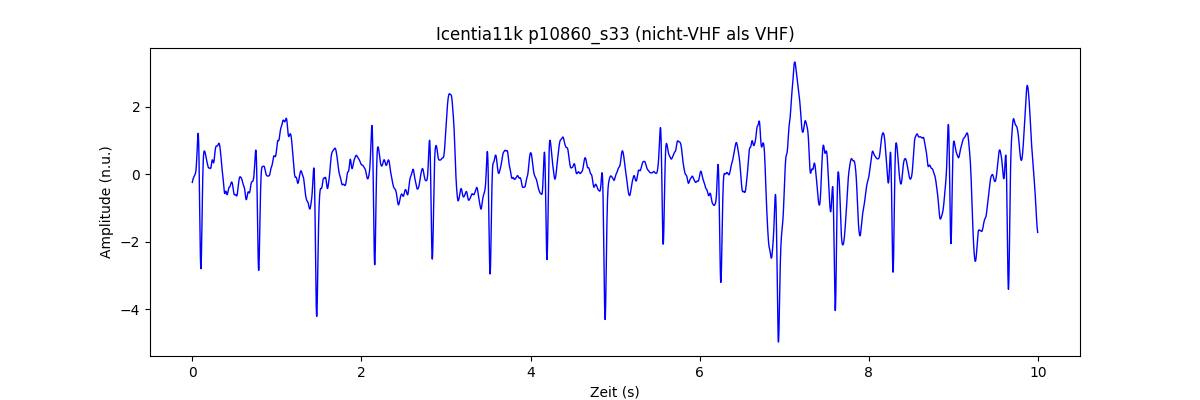
\includegraphics[width=1\textwidth]{./Bilder/icentia_verrauscht.png}
\caption[Plot einer verrauschten Icentia11k-Aufnahme]{Eine Aufnahme entnommen von Patient 10860 aus der Icentia11k-Datenbank. Sie wurde als normaler Sinusrhythmus annotiert und vom \gls{DANN} Ensemble falsch klassifiziert. Zu sehen ist, dass die Aufnahme verrauscht ist.} 
\label{fig:icentia_plot2}
\end{figure} 

\subsection*{TIMELY-Datensatz}

Das gewichtete \gls{DANN} Ensemble erzielt auf allen drei Ableitungen des TIMELY-Datensatzes einen F1-Score von 0,952-0,986, der laut \cite{plante_selection_1994} als sehr gut eingeordnet werden kann. Damit erzielt das Ensemble eine höhere Klassifikationsgüte auf einer signalmorphologisch veränderten Zieldomäne als das Modell von Ramesh et al. \cite{ramesh_atrial_2021}. Dieses Modell erreicht auf der Quelldomäne \gls{EKG} einen F1-Score von 0,93 und auf der Zieldomäne \gls{PPG}, die ein morphologisch verändertes Signal darstellt, mit Transfer Learning einen F1-Score von 0,89.

Des Weiteren erreicht das gewichtete \gls{DANN} Ensemble den bestmöglichen Recall von 1,00. Dies bedeutet, dass alle \gls{VHF}-Fälle korrekt als \gls{VHF} klassifiziert wurden. Zusammen mit einer hohen durchschnittlichen Specificity von 0,959 und einem hohen F1-Score lässt sich die Aussage treffen, dass es keine übermäßig hohen falsch positiven Klassifikationen gibt. 
Anzumerken ist hier, dass, obwohl die TIMELY-Ableitungen bei richtiger Positionierung der Elektroden modifizierte Einthoven-Ableitungen sind, dies in der Praxis nicht zutrifft. Die Morphologie der einzelnen Ableitungen variiert stark mit der Platzierung und Rotation des \gls{EKG}-Patches. Da die Patienten selbst den Patch angebracht haben, kam es vor, dass der Patch nicht über dem Herzen saß oder unter Umständen rotiert angebracht wurde, wodurch Ableitungen morphologisch verändert oder gar vertauscht sein können. Daraus lässt sich schließen, dass das Aufschlüsseln der Klassifikationsgüte nach Ableitung nicht sinnvoll ist und die Beurteilung der Klassifikationsgüte des Modells auf dem Durchschnittswert stattfinden sollte. Da auch der durchschnittliche F1-Score mit 0,973 sehr gut ist, kann Teilhypothese c) als bestätigt angesehen werden. Die Haupthypothese wurde bewiesen, da die Klassifikationsgüte des gewichteten \gls{DANN} Ensembles höher ist als die Klassifikationsgüte des gewichteten InceptionTime Ensembles (F1-Score von 0,949).

\subsection*{SHDB-AF}
Es fällt auf, dass die Klassifikationsgüte der Modelle auf der \gls{SHDB-AF} Datenbank auf der CC5-Ableitung wesentlich schlechter ist, als auf der NASA-Ableitung (F1-Scores von 0,717-0,777 vs. F1-Scores von 0,783-0,852). Die Ursache hierfür liegt darin, dass es sich bei der CC5-Ableitung um eine Brustwandableitung handelt. Für das Training der Modelle wurden nur die Ableitungen I, II, III, aVR, aVL und aVF genutzt, jedoch nicht die 6 Brustwandableitungen. Somit ist der Domain Shift zwischen den Trainingsdaten und der CC5-Ableitung der \gls{SHDB-AF} Datenbank größer als der zwischen den Trainingsdaten und der NASA-Ableitung der \gls{SHDB-AF} Datenbank und ein Abfall der Klassifikationsleistung der Modelle zu erwarten.

\begin{figure}[!ht]%
\centering
	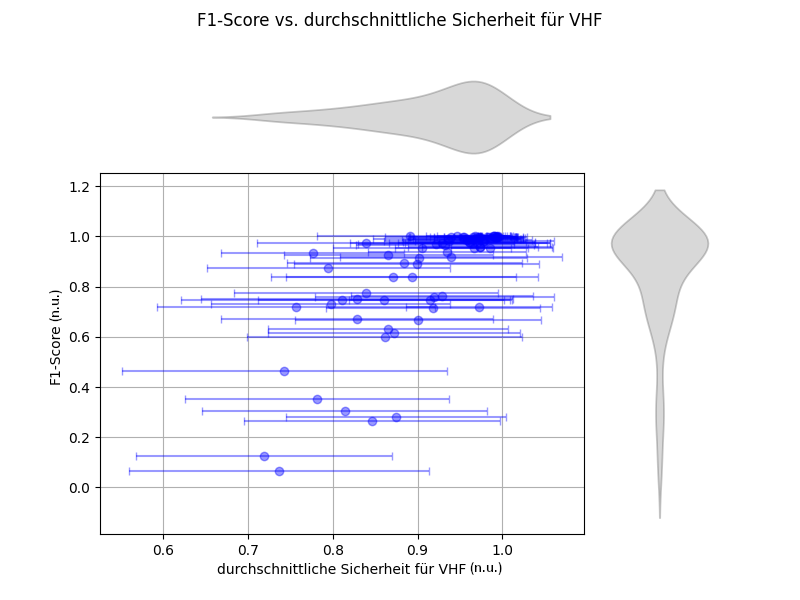
\includegraphics[width=1\textwidth]{./Bilder/shdb_plot_vhf.png}
\caption[SHDB-AF F1-Score vs. durchschnittliche Sicherheit für VHF]{F1-Score für die \gls{VHF}-Klasse gegen die durchschnittliche Sicherheit des gewichteten \gls{DANN} Ensembles pro Patient aufgetragen. Zusätzlich ist die Standardabweichung der Sicherheit pro Patient in Form von T-Balken eingetragen. Anhand des Violinenplots lässt sich die Verteilung der F1-Scores bzw. der durchschnittlichen Sicherheit für die Klassifikation über die Aufnahmen ablesen. } 
\label{fig:shdb_scatter_vhf}
\end{figure} 

Desweiteren ist die Standardabweichung der F1-Scores für \gls{VHF} innerhalb der 77 Patienten, die während der Aufzeichnung eine \gls{VHF}-Episode hatten, relativ hoch. Als Beispiel werden nun die Ergebnisse des gewichteten \gls{DANN} Ensembles auf der NASA-Ableitung betrachtet. Hier beträgt die Standardabweichung für die \gls{VHF}-Klasse 0,220. Die Standardabweichung der F1-Scores für die nicht-\gls{VHF}-Klasse innerhalb derselben 77 Patienten ist mit 0,191 vergleichbar hoch. 


In \hyperref[fig:shdb_scatter_vhf]{Abb.~7.3} ist der F1-Score für die \gls{VHF}-Klasse gegen die durchschnittliche Sicherheit des Ensembles pro Patient aufgetragen. Zusätzlich ist die Standardabweichung der Sicherheit pro Patient in Form von T-Balken eingetragen. Zu sehen ist, dass der Großteil der Teil Aufnahmen mit einem guten F1-Score und einer hohen durchschnittlichen Sicherheit klassifiziert werden konnte. Jedoch gibt es einige Patienten, deren Aufnahmen einen sehr geringen F1-Score und auch eine geringere Sicherheit in der Klassifikation aufweisen. Auf einige dieser Aufnahmen wird nun eingegangen.

\begin{figure}[!ht]%
\centering
	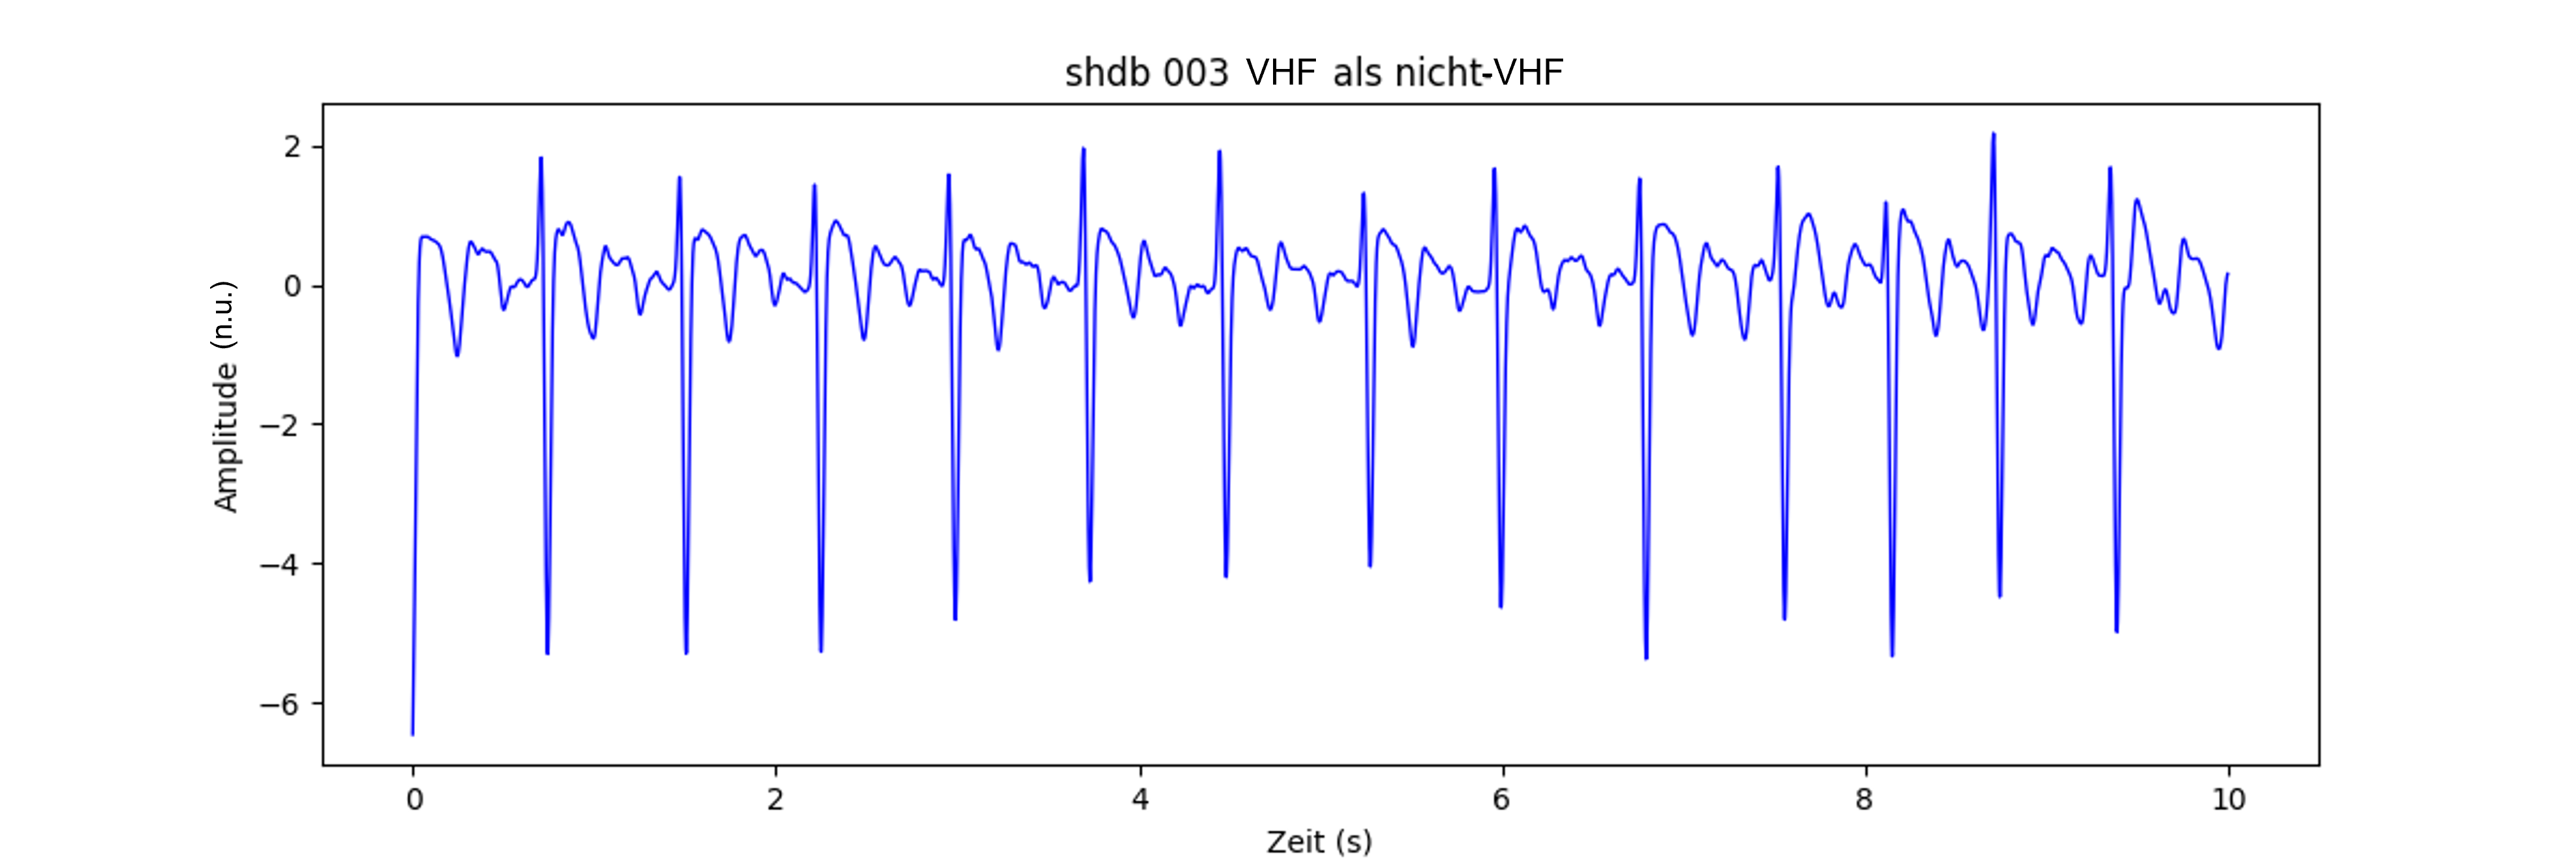
\includegraphics[width=1\textwidth]{./Bilder/003_vhf.png}
\caption[SHDB-AF Aufnahme von Patient 003 mit AFIB Annotation]{Eine Aufnahme von Patient 003 aus der SHDB-AF Datenbank, welche mit \gls{VHF} Annotiert und als nicht-\gls{VHF} vom gewichteten \gls{DANN} Ensemble klassifiziert wurde. Zu sehen ist eine regelmäßige Vorhoferregung.} 
\label{fig:shdb_003_vhf}
\end{figure} 

\begin{figure}[!ht]%
\centering
	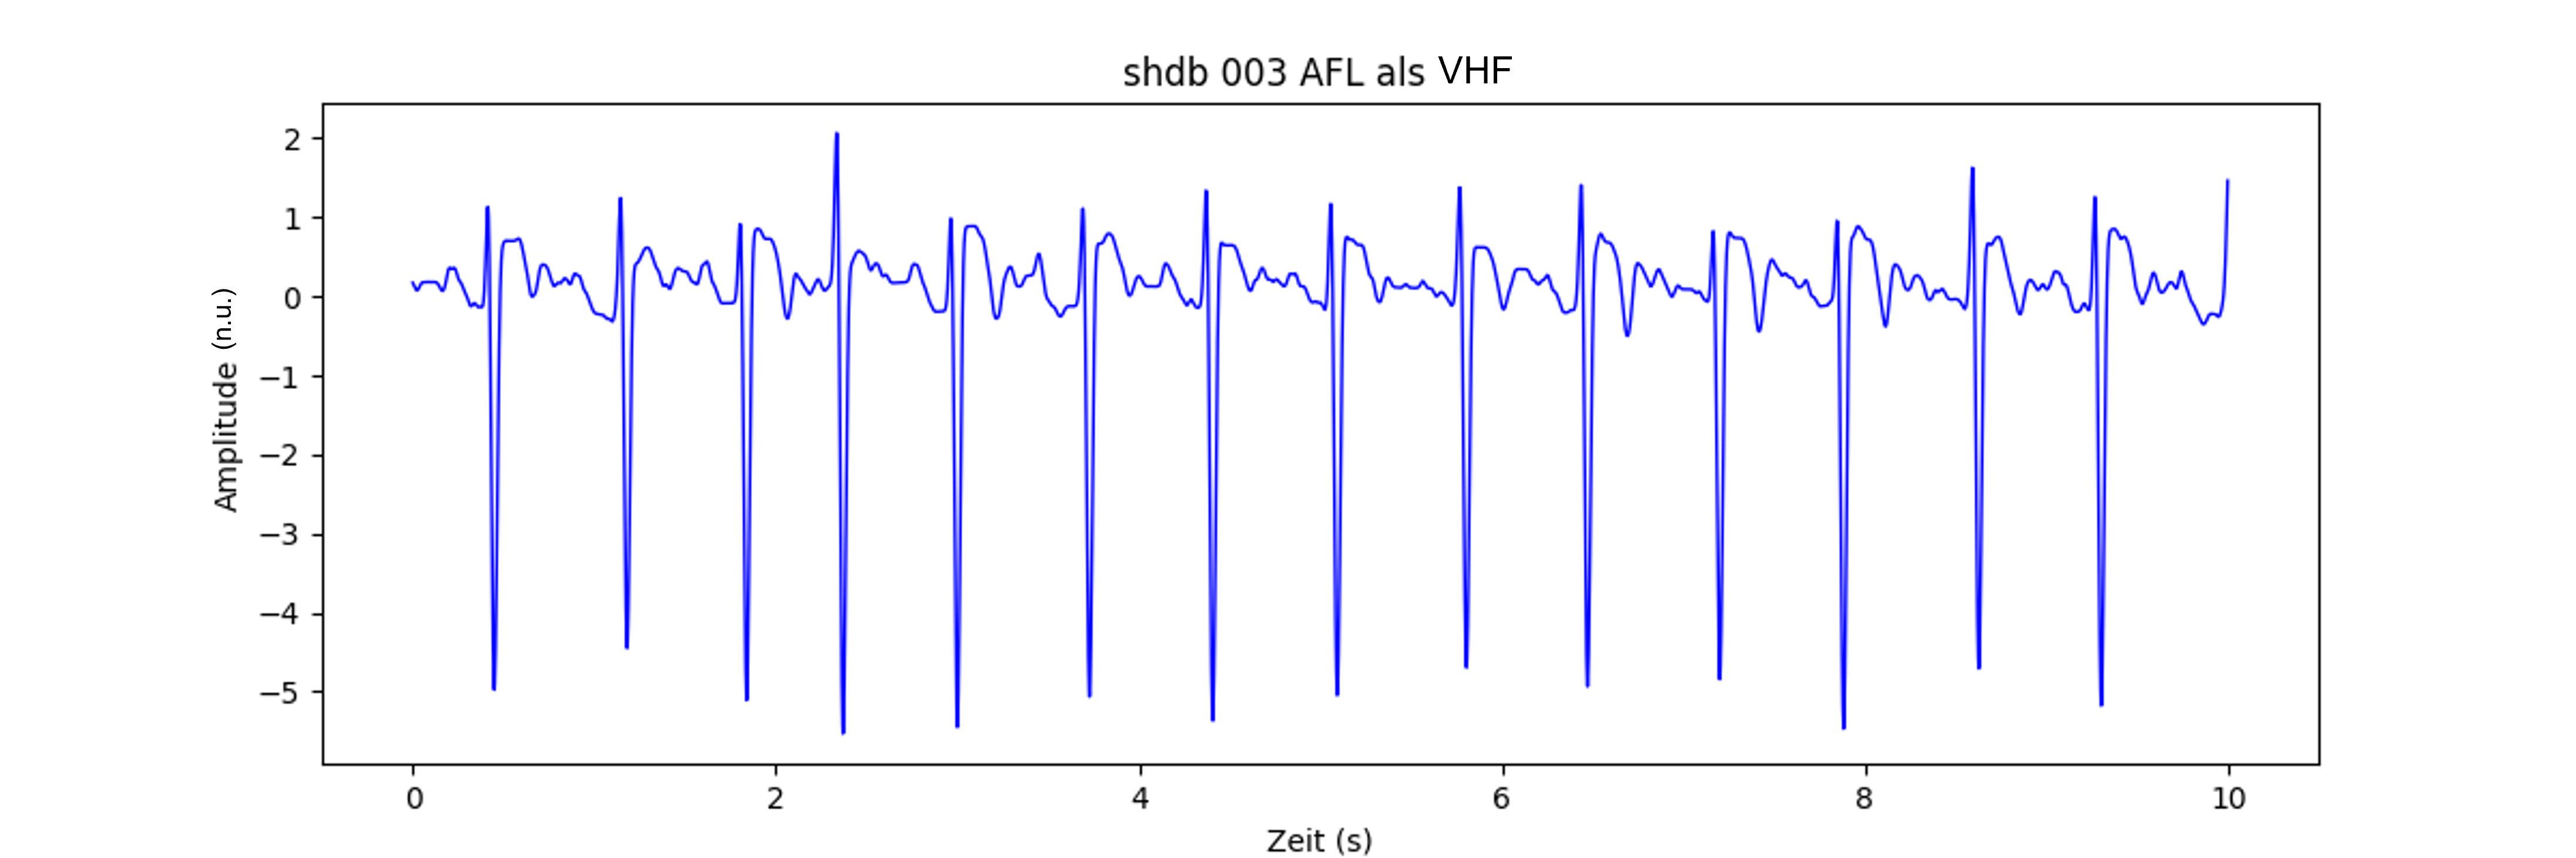
\includegraphics[width=1\textwidth]{./Bilder/003_afl.png}
\caption[SHDB-AF Aufnahme von Patient 003 mit AFL Annotation]{Eine Aufnahme von Patient 003 aus der SHDB-AF Datenbank, welche mit Vorhofflattern Annotiert und als \gls{VHF} vom gewichteten \gls{DANN} Ensemble klassifiziert wurde. Es ist keine regelmäßige Vorhoferregung zu sehen.} 
\label{fig:shdb_003_afl}
\end{figure} 

Die Klassifikation von Patient 003 erfolgte mit einem F1-Score von 0,264 für \gls{VHF} bei einer durchschnittlichen Sicherheit von 0,846. Bei diesem Patienten wurde ein mit Vorhofflattern annotierter Abschnitt vom Ensemble als \gls{VHF} klassifiziert, sowie ein mit \gls{VHF} annotierter Abschnitt nicht als \gls{VHF} detektiert. In \hyperref[fig:shdb_003_vhf]{Abb.~7.4} ist ein mit \gls{VHF} annotiertes Fenster dargestellt (welches als nicht-\gls{VHF} klassifiziert wurde), welches regelmäßige Vorhoferregungen aufweist, was auf Vorhofflattern oder Sinusrhythmus hinweist und nicht auf \gls{VHF}. In \hyperref[fig:shdb_003_afl]{Abb.~7.5} ist ein mit Vorhofflattern annotiertes Fenster dargestellt, welches als \gls{VHF} klassifiziert wurde. Hier ist keine regelmäßige Vorhoferregung zu sehen, es sind Flimmerwellen und eine leichte absolute Arrhythmie zu erkennen, sodass dies auf \gls{VHF} hinweist. Die Korrektheit der Annotationen dieser Abschnitte ist somit fraglich.


Die Klassifikation von Patient 050 erfolgte mit einem F1-Score für \gls{VHF} von 0,127 bei einer durchschnittlichen Sicherheit von 0,719. Dieser Patient besitzt insgesamt 8575 10-Sekunden-Fenster. Von diesen 8575 Fenstern sind 4 Fenster mit \gls{VHF} annotiert. Diese 4 Fenster hat das \gls{DANN} Ensemble korrekt erkannt. Auch die nicht-\gls{VHF}-Fenster wurden größtenteils korrekt klassifiziert, denn von 8571 negativen Fenstern wurden nur 55 falsch positiv klassifiziert. Durch diese starke Unausgeglichenheit der Klassen fallen jedoch selbst im Verhältnis wenige falsch positive Klassifikationen sehr stark ins Gewicht, sodass der F1-Score sehr schlecht ist. Daraus lässt sich schließen, dass der F1-Score bei unbalancierten Datensätzen keine geeignete Metrik ist.

Die Klassifikation von Patient 111 erfolgte mit einer Genauigkeit von F1~=~0,066 auf der \gls{VHF}-Klasse bei einer durchschnittlichen Sicherheit von 0,737. Bei diesem Patienten wurden Abschnitte mit Vorhoftachykardie annotiert, in denen das Ensemble \gls{VHF} detektiert. In \hyperref[fig:shdb_111_at]{Abb.~7.6} ist ein solches Fenster abgebildet. Auch hier ist die Annotation fraglich, da keine regelmäßige Vorhoferregung sichtbar und eine absolute Arrhythmie vorhanden ist.

\begin{figure}[!ht]%
\centering
	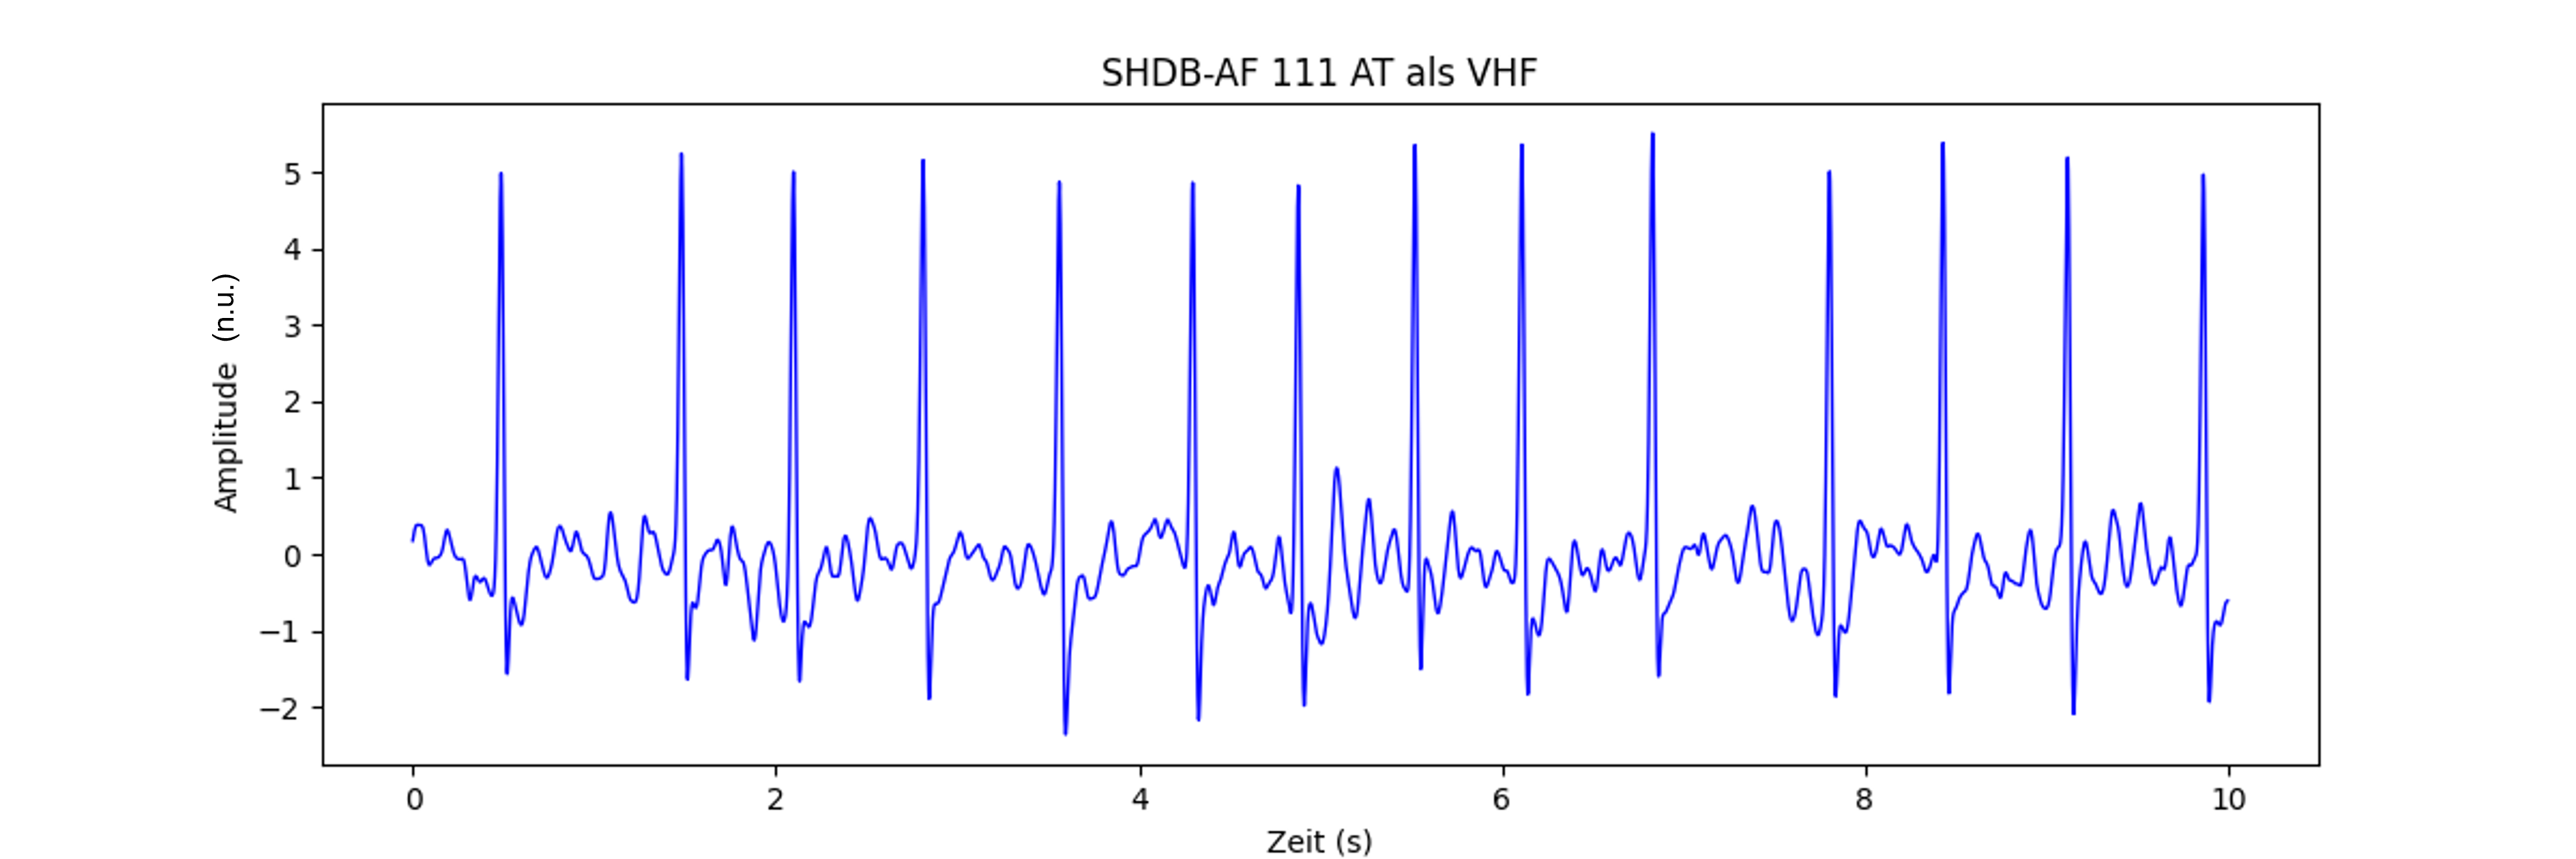
\includegraphics[width=1\textwidth]{./Bilder/111_at.png}
\caption[SHDB-AF Aufnahme von Patient 111 mit AT Annotation]{Eine Aufnahme von Patient 111 aus der SHDB-AF Datenbank, welche mit Vorhoftachkardie Annotiert und als \gls{VHF} vom gewichteten \gls{DANN} Ensemble klassifiziert wurde. Es ist keine regelmäßige Vorhoferregung zu sehen, jedoch eine absolute Arrhythmie.} 
\label{fig:shdb_111_at}
\end{figure}

\hyperref[fig:shdb_scatter_vhf]{Abb.~7.7} ist der F1-Score für die nicht-\gls{VHF}-Klasse gegen die durchschnittliche Sicherheit des Ensembles  pro Patient aufgetragen. Zusätzlich ist die Standardabweichung der Sicherheit pro Patient in Form von T-Balken eingetragen. Zu sehen ist, dass auch hier der Großteil der Teil Aufnahmen mit einem guten F1-Score und einer hohen durchschnittlichen Sicherheit klassifiziert werden konnte.

%Patient 051 hat langen Abschnitt mit N) annotiert, aber VHF detektiert (überprüfen, ob falsch annotiert)

%Patient 128 hat fast alle N abschnitte mit vhf detektiert

Die Klassifikation von Patient 024 besitzt einen F1-Score von 0,094 für die nicht-\gls{VHF}-Klasse mit einer durchschnittlichen Sicherheit von 0,606. Hier tritt derselbe Fall auf, wie bei der Klassifikation von Patient 050, mit dem Unterschied, dass Patient 024 nur drei Fenster besitzt, welche der nicht-\gls{VHF}-Klasse angehören.

Es lässt sich abschließend die Aussage treffen, dass die Klassifikation auf der SHDB-AF Datenbank zum Großteil gut funktioniert, jedoch die Gesamtgüte des Ensembles durch Aufnahmen mit einer starken Unausgeglichenheit in der Klassenverteilung und durch eventuelle falsche Annotationen reduziert wird. Aufnahmen mit einer unausgeglichenen Klassenverteilung mit vielen negativen Fällen tragen dazu bei, dass die Specificity hoch ist, da viele negative Fälle korrekt als negativ klassifiziert werden und gleichzeitig der F1-Score durch verhältnismäßig wenig falsch positive Klassifikationen verringert wird.

\begin{figure}[!ht]%
\centering
	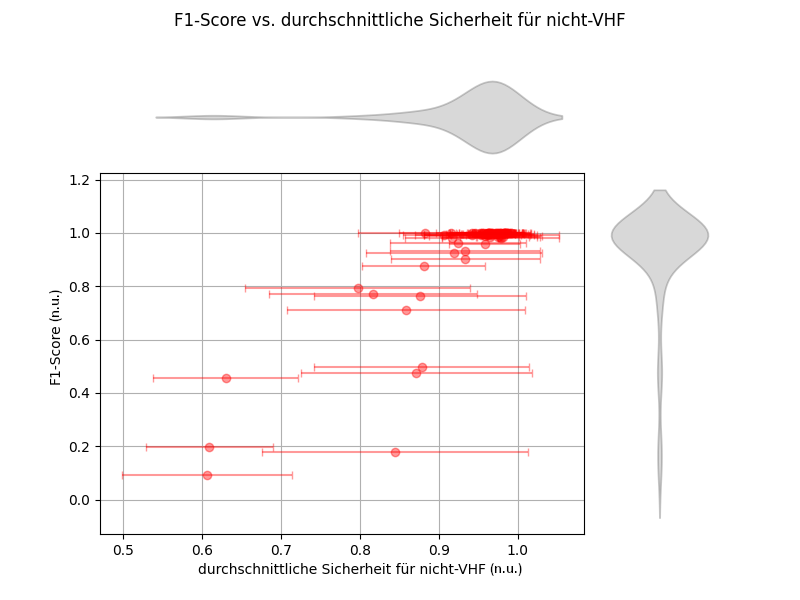
\includegraphics[width=1\textwidth]{./Bilder/shdb_plot_nicht_vhf.png}
\caption[SHDB-AF F1-Score vs. durchschnittliche Sicherheit für nicht-VHF]{F1-Score für die nicht-\gls{VHF}-Klasse gegen die durchschnittliche Sicherheit des gewichteten \gls{DANN} Ensembles pro Patient aufgetragen. Zusätzlich ist die Standardabweichung der Sicherheit pro Patient in Form von T-Balken eingetragen. Anhand des Violinenplots lässt sich die Verteilung der F1-Scores bzw. der durchschnittlichen Sicherheit für die Klassifikation über die Aufnahmen ablesen.} 
\label{fig:shdb_scatter_nvhf}
\end{figure} 

\section{Einfluss von Normalisierung}\label{sec:disknorm}

Bei der Nutzung von nicht-normalisierten Daten erzielt das gewichtete \gls{DANN} Ensemble mit einem F1-Score von 0,953 (siehe \hyperref[tab:Ergebnisse_indomain_notnorm]{Tab.~6.10}) eine minimal höhere Klassifikationsgüte auf dem Testdatensatz der Quelldomäne, als das Ensemble, welches normalisierte Daten nutzt (F1-score von 0,951, siehe \hyperref[tab:Ergebnisse_indomain]{Tab.~6.2}). Auf dem Timely Datensatz erreicht das gewichtete \gls{DANN} Ensemble ohne Normalisierung der Daten schlechtere F1-Scores (je nach Ableitung F1-Scores von 0,949-0,968 ohne Normalisierung (\hyperref[tab:Ergebnisse_timely_notnorm]{Tab.~6.11}) vs. 0,952-0,986 mit Normalisierung (\hyperref[tab:Ergebnisse_timely]{Tab.~6.6})). Daraus lässt sich schließen, dass das Unterlassen der z-Normalisierung ein Overfitting an die Trainingsdaten begünstigt. 